\documentclass{article}


% if you need to pass options to natbib, use, e.g.:
%     \PassOptionsToPackage{numbers, compress}{natbib}
% before loading AdvML_Frontiers_2024


% ready for submission for track1: regular paper
% \usepackage[track1]{AdvML_Frontiers_2024}
% ready for submission for track2: position/idea paper
% \usepackage[track2]{AdvML_Frontiers_2024}
% ready for submission for track3: demo paper
% \usepackage[track3]{AdvML_Frontiers_2024}

% to compile a camera-ready version, add the [final] option
\usepackage[final]{AdvML_Frontiers_2024}






\usepackage[utf8]{inputenc} % allow utf-8 input
\usepackage[T1]{fontenc}    % use 8-bit T1 fonts
\usepackage{hyperref}       % hyperlinks
\usepackage{url}            % simple URL typesetting
\usepackage{booktabs}       % professional-quality tables
\usepackage{amsfonts}       % blackboard math symbols
\usepackage{nicefrac}       % compact symbols for 1/2, etc.
\usepackage{microtype}      % microtypography
\usepackage{xcolor}         % colors
\usepackage{algorithm2e}
\usepackage{graphicx}
\usepackage{amsmath}


\title{Assignment 1: Enhancing Emotion Recognition Using POS Tagging}


% The \author macro works with any number of authors. There are two commands
% used to separate the names and addresses of multiple authors: \And and \AND.
%
% Using \And between authors leaves it to LaTeX to determine where to break the
% lines. Using \AND forces a line break at that point. So, if LaTeX puts 3 of 4
% authors names on the first line, and the last on the second line, try using
% \AND instead of \And before the third author name.


\author{%
  Prasanna Paithankar (21CS30065)\\
  Department of Computer Science, Indian Institute of Technology Kharagpur\\
  \texttt{paithankarprasanna@kgpian.iitkgp.ac.in} \\
  % examples of more authors
  % \And
  % Coauthor \\
  % Affiliation \\
  % Address \\
  % \texttt{email} \\
  % \AND
  % Coauthor \\
  % Affiliation \\
  % Address \\
  % \texttt{email} \\
  % \And
  % Coauthor \\
  % Affiliation \\
  % Address \\
  % \texttt{email} \\
  % \And
  % Coauthor \\
  % Affiliation \\
  % Address \\
  % \texttt{email} \\
}


\begin{document}


\maketitle


\begin{abstract}
    This document contains the implementation of a POS tagger using the Viterbi Algorithm from scratch. The POS tagger is trained on the Treebank dataset from the NLTK library. The POS tagger is then used to enhance the emotion recognition system. The emotion recognition system is trained on the Twitter messages dataset from the Hugging Face API. The system uses Tfidf for creating sentence embeddings and a classical classifier (Naive Bayes or SVM) for emotion recognition. The system is then improved by using the POS tagger to tag the dataset and augment it before sentence embedding step. The classifier is then trained again for emotion recognition using the augmented dataset. The system is evaluated on the test set of the Twitter messages dataset. The improve recognizer performs slightly better than the vanilla recognizer as presented in the classification reports and confusion matrices. The time taken for training is also presented.\\
    \\
    Assignment problem statement: \url{https://sites.google.com/view/nlp-cs-iit-kgp/assignments}
\end{abstract}


\section{POS Tagging by Viterbi Algorithm}

A bottom-up dynamic version of the Viterbi algorithm has been implemented for POS tagging on the Treebank dataset from scratch.

\begin{algorithm}
\caption{Viterbi Algorithm}
\SetAlgoLined
\KwIn{A sentence $S = w_1, w_2, w_3, ..., w_n$}
\KwOut{The most probable sequence of POS tags $T = t_1, t_2, t_3, ..., t_n$ for the sentence $S$}
\texttt{\\}
Initialization: $\pi(0, <s>, <s>) = 1$\\
\For{$k = 1$ to $n$}{
    \For{each POS tag $u$}{
        \For{each POS tag $v$}{
            $\pi(k, u, v) = \max_{w}(\pi(k-1, w, u) \times P(u|w) \times P(w|v))$\\
            $\bp(k, u, v) = \arg\max_{w}(\pi(k-1, w, u) \times P(u|w) \times P(w|v))$
        }
    }
}
$T_n = \arg\max_{u, v}(\pi(n, u, v) \times P(</s>|u) \times P(u|v))$\\
$T_{n-1} = \bp(n, T_n, </s>)$\\
\For{$k = n-2$ to $1$}{
    $T_k = \bp(k+2, T_{k+1}, T_{k+2})$
}
\end{algorithm}

\subsection{Computing Transition and Emission Probabilities}

The transition and emission probabilities are computed using the Treebank dataset. The transition probability $P(u|v)$ is the probability of a POS tag $u$ given the previous POS tag $v$. The emission probability $P(w|v)$ is the probability of a word $w$ given the POS tag $v$. The probabilities are computed as follows:

\begin{equation}
    P(u|v) = \frac{C(v, u)}{C(v)}
\end{equation}

\begin{equation}
    P(w|v) = \frac{C(v, w)}{C(v)}
\end{equation}
    
    where $C(v, u)$ is the count of the POS tag $u$ following the POS tag $v$, $C(v, w)$ is the count of the word $w$ with the POS tag $v$, and $C(v)$ is the count of the POS tag $v$.

In the final implementation, we apply smoothing to the probabilities to handle unseen words and POS tags.

\begin{equation}
    P(u|v) = \frac{C(v, u) + \epsilon}{C(v) + \epsilon \times |V|}
\end{equation}

\begin{equation}
    P(w|v) = \frac{C(v, w) + \epsilon}{C(v) + \epsilon \times |V|}
\end{equation}
    
    where $|V|$ is the size of the vocabulary and $\epsilon$ is a smoothing hyper-parameter.

\subsection{Results}
We evaluate the implemented POS tagger on the Treebank dataset and compare the results with the NLTK POS tagger. Time benchmarked on 11th Gen Intel(R) Core(TM) i5-1135G7 @ 2.40GHz, 2401 Mhz, 4 Core(s), 8 Logical Processor(s).

\renewcommand{\arraystretch}{1.5}
\begin{table}[h]
\centering
\begin{tabular}{|c|c|c|}
\hline
\textbf{POS Tagger} & \textbf{Accuracy} & \textbf{Time (s)} \\ \hline
viterbi         & 0.97162              & 104           \\ \hline
nltk.pos\_tag                & 0.89298              & 3            \\ \hline
\end{tabular}
\bigskip
\caption{POS Tagging Results}
\end{table}

Some sample POS tagging results are presented in the \hyperref[appendix]{Appendix}.


\section{Vanilla Emotion Recognizer}

The Twitter messages corpus is loaded using the Hugging Face API. The dataset is split into training, validation, and test sets. The corpus has 6 labels: joy, sadness, anger, fear, love, and surprise. We perform a multi-class classification on the training set and evaluate the model on the test set.

\subsection{Data Preprocessing and Vectorization}
The text data is preprocessed by lemmatizing the words. Lemmatization is implemented as WordNet Lemmatizer from the NLTK library. The text data is then vectorized using Tfidf to create sentence embeddings.

\subsection{Naive Bayes Classifier}
Naive Bayes classifier is implemented as sklearn.naive\_bayes.MultinomialNB. The classifier is trained on the training set and evaluated on the test set.

Training time: 0s

The results are presented in \hyperref[table:nb_results_1]{Table 2} and \hyperref[fig:nb_confusion_matrix_1]{Figure 1}.

\begin{table}[h]
    \label{table:nb_results_1}
\centering
\begin{tabular}{|c|c|c|c|c|c|}
\hline
\textbf{Label} & \textbf{Precision} & \textbf{Recall} & \textbf{F1-score} & \textbf{Support} \\ \hline
sadness        & 0.68               & 0.92            & 0.78              & 581              \\ \hline
joy            & 0.62               & 0.99            & 0.76              & 695              \\ \hline
love           & 1.00               & 0.03            & 0.05              & 159              \\ \hline
anger          & 0.94               & 0.19            & 0.31              & 275              \\ \hline
fear           & 1.00               & 0.19            & 0.32              & 224              \\ \hline
surprise       & 0.00               & 0.00            & 0.00              & 66               \\ \hline
 &  &  &  &  \\ \hline
accuracy       &                     &                 & 0.66              & 2000             \\ \hline
macro avg      & 0.71               & 0.38            & 0.37              & 2000             \\ \hline
weighted avg   & 0.73               & 0.66            & 0.57              & 2000             \\ \hline
\end{tabular}
\bigskip
\caption{Naive Bayes Classifier Results}
\end{table}

\begin{figure}[h]
    \label{fig:nb_confusion_matrix_1}
    \centering
    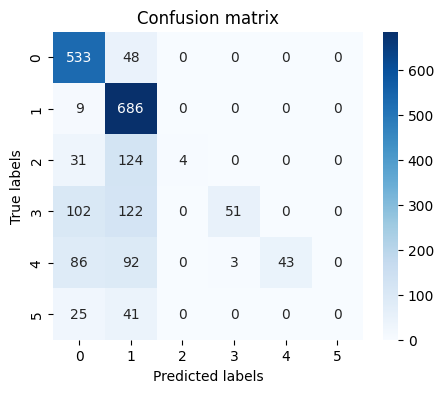
\includegraphics[width=0.5\textwidth]{confusion_matrix_2_nb.png}
    \caption{Confusion Matrix for Naive Bayes Classifier}
\end{figure}

\subsection{SVM Classifier}
SVM classifier is implemented as sklearn.svm.SVC. The classifier is trained on the training set and evaluated on the test set.

Training time: 125s

The results are presented in \hyperref[table:svm_results_1]{Table 3} and \hyperref[fig:svm_confusion_matrix_1]{Figure 2}.

\begin{table}[h]
    \label{table:svm_results_1}
\centering
\begin{tabular}{|c|c|c|c|c|c|}
\hline
\textbf{Label} & \textbf{Precision} & \textbf{Recall} & \textbf{F1-score} & \textbf{Support} \\ \hline
sadness        & 0.89               & 0.93            & 0.91              & 581              \\ \hline
joy            & 0.82               & 0.96            & 0.88              & 695              \\ \hline
love           & 0.87               & 0.54            & 0.67              & 159              \\ \hline
anger          & 0.90               & 0.79            & 0.84              & 275              \\ \hline
fear           & 0.86               & 0.78            & 0.82              & 224              \\ \hline
surprise       & 0.85               & 0.44            & 0.58              & 66               \\ \hline
&  &  &  & \\ \hline
accuracy       &                     &                 & 0.86              & 2000             \\ \hline
macro avg      & 0.86               & 0.74            & 0.78              & 2000             \\ \hline
weighted avg   & 0.86               & 0.86            & 0.85              & 2000             \\ \hline
\end{tabular}
\bigskip
\caption{SVM Classifier Results}
\end{table}

\begin{figure}[h]
    \label{fig:svm_confusion_matrix_1}
    \centering
    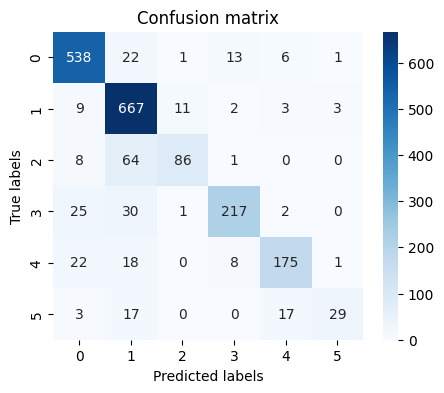
\includegraphics[width=0.5\textwidth]{confusion_matrix_2_svm.png}
    \caption{Confusion Matrix for SVM Classifier}
\end{figure}

\section{Improved Emotion Recognizer}

The corpus is augmented using the POS tagger implemented in the previous section. We present the pipeline for the same and two augmentation strategies.

\subsection{Pipeline}
\begin{algorithm}
\caption{Improved Emotion Recognizer Pipeline}
\SetAlgoLined
\KwIn{A sentence $S = w_1, w_2, w_3, ..., w_n$}
\KwIn{POS tag classes $C = c_1, c_2, c_3, ..., c_m$}
\KwOut{The most probable emotion label $E$ for the sentence $S$}
\texttt{\\}
POS tagging: $T = t_1, t_2, t_3, ..., t_n$\\
Filtering: $S' = w_i \text{ if } t_i \in C$\\
Tfidf Vectorization: $X = \text{Tfidf}(S')$\\
Train the model: $M = \text{Classifier}(X)$\\
Predict the emotion label: $E = M.predict(X)$
\end{algorithm}

\subsection{Augmentation}
The POS tagger is used to tag the Twitter messages dataset. We manually select the POS tag classes that are relevant for emotion recognition. The POS tag classes are used to filter the words in the dataset. The filtered words are then used to create sentence embeddings using Tfidf.

We use the following POS tag classes for augmentation: {'<s>', '-LRB-', 'NN', 'JJR', 'NNP', 'VBZ', 'RB', "''", '</s>', 'VBN', 'RBS', 'VB', 'NNPS', '-RRB-', 'NNS', 'PDT', 'JJ', 'VBP', 'RP', 'VBG', 'RBR', 'FW', 'VBD', 'WDT', 'WRB', '-NONE-', 'WP', 'POS', 'JJS', '``', 'WP\$', 'UH'}

\subsection{Alternative Augmentation Strategy}
(This has not been implemented in the final code)

We consider words which have ambiguous POS tags. We take such words and replace them with a synonym using nltk.corpus.wordnet.synsets. We then use the POS tagger to tag the augmented dataset after removing stopwords.

\subsubsection{Naive Bayes Classifier}
Naive Bayes classifier is trained on the augmented dataset and evaluated on the test set.

Training time: 0s

The results are presented in \hyperref[table:nb_results_3]{Table 4} and \hyperref[fig:nb_confusion_matrix_3]{Figure 3}.

\begin{table}[h]
    \label{table:nb_results_3}
\centering
\begin{tabular}{|c|c|c|c|c|c|}
\hline
\textbf{Label} & \textbf{Precision} & \textbf{Recall} & \textbf{F1-score} & \textbf{Support} \\ \hline
sadness            & 0.68               & 0.93            & 0.79              & 581              \\ \hline
joy        & 0.64               & 0.98            & 0.78              & 695              \\ \hline
love          & 1.00               & 0.04            & 0.08              & 159              \\ \hline
anger           & 0.94               & 0.27            & 0.41              & 275              \\ \hline
fear           & 0.92               & 0.25            & 0.39              & 224              \\ \hline
surprise       & 0.00               & 0.00            & 0.00              & 66               \\ \hline
&  &  &  &  \\ \hline
accuracy       &                     &                 & 0.68              & 2000             \\ \hline
macro avg      & 0.70               & 0.41            & 0.41              & 2000             \\ \hline
weighted avg   & 0.73               & 0.68            & 0.61              & 2000             \\ \hline
\end{tabular}
\bigskip
\caption{Naive Bayes Classifier Results on Augmented Dataset}
\end{table}

\begin{figure}[h]
    \label{fig:nb_confusion_matrix_3}
    \centering
    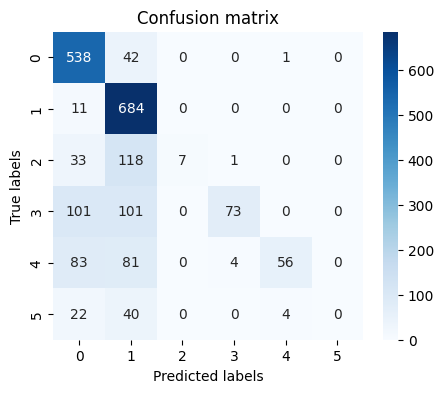
\includegraphics[width=0.5\textwidth]{confusion_matrix_3_nb.png}
    \caption{Confusion Matrix for Naive Bayes Classifier on Augmented Dataset}
\end{figure}

\subsubsection{SVM Classifier}
SVM classifier is trained on the augmented dataset and evaluated on the test set.

Training time: 108s

The results are presented in \hyperref[table:svm_results_3]{Table 5} and \hyperref[fig:svm_confusion_matrix_3]{Figure 4}.

\begin{table}[h]
    \label{table:svm_results_3}
\centering
\begin{tabular}{|c|c|c|c|c|c|}
\hline
\textbf{Label} & \textbf{Precision} & \textbf{Recall} & \textbf{F1-score} & \textbf{Support} \\ \hline
sadness        & 0.90               & 0.92            & 0.91              & 581              \\ \hline
joy            & 0.81               & 0.96            & 0.88              & 695              \\ \hline
love           & 0.87               & 0.53            & 0.66              & 159              \\ \hline
anger          & 0.90               & 0.79            & 0.84              & 275              \\ \hline
fear           & 0.87               & 0.79            & 0.82              & 224              \\ \hline
surprise       & 0.85               & 0.50            & 0.63              & 66               \\ \hline
&  &  &  &  \\ \hline
accuracy       &                     &                 & 0.86              & 2000             \\ \hline
macro avg      & 0.87               & 0.75            & 0.79              & 2000             \\ \hline
weighted avg   & 0.86               & 0.86            & 0.85              & 2000             \\ \hline
\end{tabular}
\bigskip
\caption{SVM Classifier Results on Augmented Dataset}
\end{table}

\begin{figure}[h]
    \label{fig:svm_confusion_matrix_3}
    \centering
    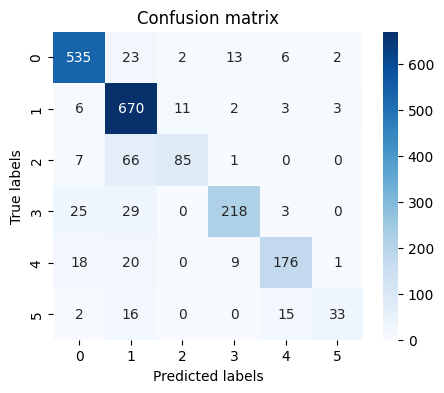
\includegraphics[width=0.5\textwidth]{confusion_matrix_3_svm.png}
    \caption{Confusion Matrix for SVM Classifier on Augmented Dataset}
\end{figure}

\section{Comparison}
The results of the vanilla and improved emotion recognizers are compared in the \hyperref[table:comparison]{Table 6}.
\begin{table}[h]
    \label{table:comparison}
\centering
\begin{tabular}{|c|c|c|c|}
\hline
\textbf{Classifier} & \textbf{Accuracy} & \textbf{Macro average F1-score} & \textbf{Training time (s)} \\ \hline
Naive Bayes (Vanilla) & 0.66 & 0.37 & 0 \\ \hline
Naive Bayes (Improved) & 0.68 & 0.41 & 0 \\ \hline
SVM (Vanilla) & 0.86 & 0.78 & 125 \\ \hline
SVM (Improved) & 0.86 & 0.79 & 108 \\ \hline
\end{tabular}
\bigskip
\caption{Comparison of Vanilla and Improved Emotion Recognizers}
\end{table}

\section{Conclusion}
We have implemented a POS tagger using the Viterbi Algorithm from scratch. The POS tagger is trained on the Treebank dataset and evaluated (97\%) giving better results than nltk.pos\_tag (89\%). We then implement an emotion recognition system using the Twitter messages dataset. The system uses Tfidf for creating sentence embeddings and a classical classifier (Naive Bayes or SVM) for emotion recognition. The system is then improved by augmenting the dataset using the POS tagger. The classifier is trained again for emotion recognition using the augmented dataset. The system is evaluated on the test set of the Twitter messages dataset. We find slight improvement in the performance of the improved recognizer as compared to the vanilla recognizer.


%%%%%%%%%%%%%%%%%%%%%%%%%%%%%%%%%%%%%%%%%%%%%%%%%%%%%%%%%%%%
% start from new page
\clearpage

\appendix

\section{Viterbi Tagging Samples}
\label{appendix}
Format: [(Word, Actual tag, Predicted tag), ... ]

1. [('Pierre', 'NNP', 'NNP'), ('Vinken', 'NNP', 'NNP'), (',', ',', ','), ('61', 'CD', 'CD'), ('years', 'NNS', 'NNS'), ('old', 'JJ', 'JJ'), (',', ',', ','), ('will', 'MD', 'MD'), ('join', 'VB', 'VB'), ('the', 'DT', 'DT'), ('board', 'NN', 'NN'), ('as', 'IN', 'IN'), ('a', 'DT', 'DT'), ('nonexecutive', 'JJ', 'JJ'), ('director', 'NN', 'NN'), ('Nov.', 'NNP', 'NNP'), ('29', 'CD', 'CD'), ('.', '.', '.')]

2. [('Mr.', 'NNP', 'NNP'), ('Vinken', 'NNP', 'NNP'), ('is', 'VBZ', 'VBZ'), ('chairman', 'NN', 'NN'), ('of', 'IN', 'IN'), ('Elsevier', 'NNP', 'NNP'), ('N.V.', 'NNP', 'NNP'), (',', ',', ','), ('the', 'DT', 'DT'), ('Dutch', 'NNP', 'JJ'), ('publishing', 'VBG', 'NN'), ('group', 'NN', 'NN'), ('.', '.', '.')]

3. [('Rudolph', 'NNP', 'NNP'), ('Agnew', 'NNP', 'NNP'), (',', ',', ','), ('55', 'CD', 'CD'), ('years', 'NNS', 'NNS'), ('old', 'JJ', 'JJ'), ('and', 'CC', 'CC'), ('former', 'JJ', 'JJ'), ('chairman', 'NN', 'NN'), ('of', 'IN', 'IN'), ('Consolidated', 'NNP', 'NNP'), ('Gold', 'NNP', 'NNP'), ('Fields', 'NNP', 'NNP'), ('PLC', 'NNP', 'NNP'), (',', ',', ','), ('was', 'VBD', 'VBD'), ('named', 'VBN', 'VBN'), ('*-1', '-NONE-', '-NONE-'), ('a', 'DT', 'DT'), ('nonexecutive', 'JJ', 'JJ'), ('director', 'NN', 'NN'), ('of', 'IN', 'IN'), ('this', 'DT', 'DT'), ('British', 'JJ', 'JJ'), ('industrial', 'JJ', 'JJ'), ('conglomerate', 'NN', 'NN'), ('.', '.', '.')]

4. [('A', 'DT', 'DT'), ('form', 'NN', 'NN'), ('of', 'IN', 'IN'), ('asbestos', 'NN', 'NN'), ('once', 'RB', 'RB'), ('used', 'VBN', 'VBN'), ('*', '-NONE-', '-NONE-'), ('*', '-NONE-', '-NONE-'), ('to', 'TO', 'TO'), ('make', 'VB', 'VB'), ('Kent', 'NNP', 'NNP'), ('cigarette', 'NN', 'NN'), ('filters', 'NNS', 'NNS'), ('has', 'VBZ', 'VBZ'), ('caused', 'VBN', 'VBN'), ('a', 'DT', 'DT'), ('high', 'JJ', 'JJ'), ('percentage', 'NN', 'NN'), ('of', 'IN', 'IN'), ('cancer', 'NN', 'NN'), ('deaths', 'NNS', 'NNS'), ('among', 'IN', 'IN'), ('a', 'DT', 'DT'), ('group', 'NN', 'NN'), ('of', 'IN', 'IN'), ('workers', 'NNS', 'NNS'), ('exposed', 'VBN', 'VBN'), ('*', '-NONE-', '-NONE-'), ('to', 'TO', 'TO'), ('it', 'PRP', 'PRP'), ('more', 'RBR', 'JJR'), ('than', 'IN', 'IN'), ('30', 'CD', 'CD'), ('years', 'NNS', 'NNS'), ('ago', 'IN', 'RB'), (',', ',', ','), ('researchers', 'NNS', 'NNS'), ('reported', 'VBD', 'VBD'), ('0', '-NONE-', '-NONE-'), ('*T*-1', '-NONE-', '-NONE-'), ('.', '.', '.')]

5. [('The', 'DT', 'DT'), ('asbestos', 'NN', 'NN'), ('fiber', 'NN', 'NN'), (',', ',', ','), ('crocidolite', 'NN', 'NN'), (',', ',', ','), ('is', 'VBZ', 'VBZ'), ('unusually', 'RB', 'RB'), ('resilient', 'JJ', 'JJ'), ('once', 'IN', 'IN'), ('it', 'PRP', 'PRP'), ('enters', 'VBZ', 'VBZ'), ('the', 'DT', 'DT'), ('lungs', 'NNS', 'NNS'), (',', ',', ','), ('with', 'IN', 'IN'), ('even', 'RB', 'RB'), ('brief', 'JJ', 'JJ'), ('exposures', 'NNS', 'NNS'), ('to', 'TO', 'TO'), ('it', 'PRP', 'PRP'), ('causing', 'VBG', 'VBG'), ('symptoms', 'NNS', 'NNS'), ('that', 'WDT', 'WDT'), ('*T*-1', '-NONE-', '-NONE-'), ('show', 'VBP', 'VBP'), ('up', 'RP', 'RP'), ('decades', 'NNS', 'NNS'), ('later', 'JJ', 'JJ'), (',', ',', ','), ('researchers', 'NNS', 'NNS'), ('said', 'VBD', 'VBD'), ('0', '-NONE-', '-NONE-'), ('*T*-2', '-NONE-', '-NONE-'), ('.', '.', '.')]



%%%%%%%%%%%%%%%%%%%%%%%%%%%%%%%%%%%%%%%%%%%%%%%%%%%%%%%%%%%%


\end{document}